\documentclass{article}

\PassOptionsToPackage{authoryear,square}{natbib}
\usepackage[final]{neurips_2026}
\usepackage[T1]{fontenc}
\usepackage{amsmath}
\usepackage{amssymb}
\usepackage{booktabs}
\usepackage{tabularx}
\usepackage{graphicx}
\usepackage{caption}
\usepackage{float}
\usepackage{enumitem}
\usepackage{xcolor}
\definecolor{citeblue}{HTML}{1D4E89}
\usepackage[colorlinks=true,citecolor=citeblue,linkcolor=black,urlcolor=citeblue]{hyperref}
\usepackage{microtype}

\graphicspath{{../output/report/figures/}{output/report/figures/}}

\setlist[itemize]{leftmargin=1.5em,itemsep=0.2ex,topsep=0.4ex}
\captionsetup{font=small,labelfont=bf}
\setcitestyle{authoryear,square}
\makeatletter
\renewcommand{\@noticestring}{AI Alignment Final Project Report.}
\makeatother
\raggedbottom

\title{Cross-Modal Observational Learning with Intent-Like Representations from Reward-Free Pretraining}
\author{Huo Bingnan\thanks{The author worked alone and was responsible for the project idea, implementation, experiments, presentation, and report.}}
\date{}

\begin{document}
\maketitle

\begin{abstract}
Observational learning asks whether an agent can learn useful behavioral structure by watching others act and later reuse that structure through its own controller. I study a controlled version of this question: can observation-derived, intent-like representations be grounded across a visual/state modality gap and used inside an offline control pipeline? Starting from InFOM, an intention-conditioned offline RL method with reward-free pretraining, I implement two cross-modal bridge variants on paired RGB/state data. Pretraining is the central stage: it learns both the observation-to-control bridge and the InFOM-style latent structure before reward-labeled fine-tuning. The state-distilled variant gives stronger best-checkpoint control signals than a contrastive alignment variant, but final-window success remains unstable. The result is a narrow proof of concept: paired cross-modal grounding can make observation-derived representations partially useful for control, while the broader goals of unpaired observation transfer, semantic intent inference, and causal-effect learning remain open.
\end{abstract}

\section{Introduction}

Agents often learn not only by acting, but also by watching others interact with the world. This ability, usually described as observational learning, suggests that useful behavioral structure can be extracted before the learner performs the task itself \citep{Bandura1977}. Developmental psychology makes the goal-directed part of this especially concrete: infants can re-enact what an adult intended to do even when the adult visibly failed \citep{Meltzoff1995}.

The same question matters in robotics and embodied AI. Many successful imitation-learning systems rely on demonstrations collected through the learner's own control interface, such as robot teleoperation \citep{Osa2018,Fu2024MobileALOHA}. Such data can be powerful, but it is also expensive, embodiment-specific, and difficult to scale \citep{Fu2024MobileALOHA}. Observation is easier to obtain, yet not automatically usable for control: the learner may see a different state representation, lack the teacher's actions, or act through a different body. I therefore view observational learning as a complement to reinforcement learning, planning, and direct demonstrations, not as a replacement for them \citep{Borsa2019,Chang2024ILfO}.

Observed trajectories contain at least two useful levels of structure. A learner can infer low-level action patterns, meaning what controls appear to produce the observed motion. It can also infer a higher-level intent, goal, or effect, meaning what the actor is trying to make happen. For example, when a car changes lanes, accelerates past a slower car, and returns to its lane, the visible motion suggests both a sequence of actions and the intent to overtake. Failed attempts can also reveal an intended effect. Causal effect learning is only a motivation here, but it points to why observational learning should go beyond view alignment or action copying.

The project asks whether intent-like abstractions learned from observation can be reused for control. The full version of this question includes unpaired observation, semantic goal inference, cross-embodiment transfer, and causal reasoning. I focus on a tractable proxy: whether paired cross-modal grounding can connect observation-derived representations to an InFOM-style offline RL pipeline. InFOM is a useful starting point because it already separates reward-free pretraining, where latent intention and flow-occupancy structure are learned, from reward-labeled fine-tuning. I extend that separation by making pretraining also learn the cross-modal RGB/state bridge.

The original hypotheses were broader than the final implementation. H1 proposed that third-person trajectories contain enough information to infer temporally extended intent without aligned first-person state-action pairs. H2 proposed that a shared latent can align third-person and first-person behavior while capturing strategy rather than viewpoint or identity. H3 proposed that conditioning a first-person policy on this latent improves learning over state-only and non-intent observational baselines. The final experiments measure progress toward these hypotheses in a paired bridge setting, rather than fully testing unpaired transfer or semantic intent inference.

Concretely, reward-free pretraining uses paired state/RGB transitions; reward-labeled fine-tuning uses third-person-view (TPV) RGB observations in the grounded latent space; and deployment/evaluation uses the learner-side low-dimensional state path to produce actions. This extends InFOM beyond its original shared-interface setting, but it remains a proof of concept. InFOM's ``intention'' is an operational future-occupancy latent, not the full semantic or causal notion of intent motivating the project.

The contributions are:
\begin{itemize}[leftmargin=1.5em]
    \item a controlled formulation of observational learning as cross-modal grounding for intent-like control representations;
    \item two InFOM bridge variants that use reward-free pretraining to learn observation-to-control grounding;
    \item an empirical audit showing stronger control signals from state distillation than from contrastive alignment alone, with fine-tuning instability as the main limitation.
\end{itemize}

\section{Related Work}

\paragraph{Imitation, behavior cloning, and third-person alignment.}
Imitation learning and behavior cloning usually assume demonstrations in the learner's own interface: observations are paired with expert actions in the same state, sensor, and action space used by the policy \citep{Osa2018}. Teleoperation systems such as Mobile ALOHA satisfy this assumption by collecting robot-operated demonstrations that already match deployment \citep{Fu2024MobileALOHA}. The setting here keeps the observation/control gap explicit: reward-free bridge data connects TPV RGB to learner-side state/action transitions, and reward-labeled TPV data must later become useful for learner-side control. Third-person imitation, Time-Contrastive Networks, and XIRL relax parts of the interface assumption through viewpoint, embodiment, or visual-domain alignment \citep{Stadie2017ThirdPerson,Sermanet2018TCN,Zakka2022XIRL}. Method B uses a related paired alignment step, but only as pretraining for an InFOM-style offline RL pipeline rather than as the final imitation objective.

\paragraph{Cross-embodiment skill transfer.}
MimicPlay and UniSkill are close in motivation because they transfer structure from richer human or cross-embodiment observations to robot behavior \citep{Wang2023MimicPlay,Kim2025UniSkill}. MimicPlay uses human-play latent plans to guide policies trained on robot teleoperation, while UniSkill extracts skills from cross-embodiment videos and conditions robot policies on them. In contrast, the diagnostic question here is narrower: can reward-free paired bridge data make TPV representations usable inside an offline RL pipeline when reward-labeled data are TPV observations rather than direct learner-side state observations?

\paragraph{Latent intentions, offline RL, and reward learning.}
InFOM is the direct algorithmic backbone \citep{Zheng2025InFOM}. It pretrains an intention encoder and SARSA flow occupancy model from reward-free state/action transitions, then uses reward-labeled data to learn reward, critic, and policy components. Its ``intention'' is a latent variable for explaining heterogeneous future occupancy under a consistency assumption over adjacent transitions, not a guaranteed semantic goal or causal effect. Passive-data latent-intention methods such as ICVF similarly study how passive or reward-free data can support downstream RL \citep{Ghosh2023ICVF}. I keep InFOM's pretraining/fine-tuning split but change the interface assumption: pretraining must also learn a bridge from TPV observations into a learner-side control representation.

\paragraph{Inverse reinforcement learning.}
Inverse reinforcement learning uses observation to infer a reward function and then optimize it \citep{NgRussell2000IRL}. T-REX is especially relevant because it learns reward from ranked suboptimal demonstrations and can extrapolate beyond poor demonstrations \citep{Brown2019TREX}. Here, rewards are provided during fine-tuning; the question is whether cross-modal latent grounding can make reward-labeled TPV observations useful for offline control.

\section{Problem Formulation}

Let a teacher or observed actor generate a trajectory
\begin{equation}
    \tau^T = (o^T_0, a^T_0, o^T_1, a^T_1, \ldots, o^T_H),
\end{equation}
where some components, especially $a^T_t$, may be unavailable. The learner acts through its own interface,
\begin{equation}
    x^L_t \in \mathcal{X}^L, \qquad a^L_t \in \mathcal{A}^L,
\end{equation}
which may differ from the teacher's. The broad goal is to infer an intent/effect latent
\begin{equation}
    z \sim q_\phi(z \mid \tau^T),
\end{equation}
that captures what the teacher is trying to accomplish and can condition a learner policy,
\begin{equation}
    \pi_\theta(a^L_t \mid x^L_t, z),
\end{equation}
so the learner can cause the corresponding effect in its own environment. This is the conceptual target; the implementation uses InFOM's latent-intention machinery and a grounded learner-side state path as a controlled proxy.

This formulation separates three coupled problems: grounding observations into the learner's interface, inferring an intent/effect beyond visible motion, and realizing that effect through learner actions. Useful observational learning needs both a representation bridge and a temporally extended signal that can support control. The experiments focus on the bridge and an InFOM-style proxy for the second part.

The bridge version uses reward-free paired learner-side state, TPV RGB, and action transitions. Reward-labeled fine-tuning then uses TPV RGB after grounding, while deployment/evaluation samples actions through the learner-side low-dimensional state path. This isolates whether pretraining can turn observation-side data into a representation that a later control pipeline can use.

\section{Method and Experimental Setup}

\subsection{High-Level Method Concept}

The method has two linked parts: a cross-modal grounding model and an InFOM-style latent-intention model. Both are learned during reward-free pretraining, so pretraining is where observation-side data become usable by the later control pipeline. Let $E_T$ encode teacher-side observations and $E_L$ encode the learner-side interface. The grounding goal is to map both into a shared latent space:
\begin{equation}
    h^T_t = E_T(o^T_t), \qquad h^L_t = E_L(x^L_t).
\end{equation}
With paired or weakly aligned observations, a grounding loss encourages the latents to represent the same state, effect, or behavioral situation:
\begin{equation}
    \mathcal{L}_{\mathrm{ground}} =
    d(h^T_t, h^L_t) + d(h^T_{t+1}, h^L_{t+1}).
\end{equation}
The intent-conditioned part introduces a latent variable for temporally extended behavior,
\begin{equation}
    \eta \sim q_\phi(\eta \mid h_{t+1}, a_{t+1}),
\end{equation}
and learns future latent occupancy conditioned on the current latent, action, and intent proxy. Pretraining jointly learns the latent structure, behavior-cloning actor, and grounding losses before rewards are introduced. Reward-labeled fine-tuning then tests whether these representations support reward, critic, flow, and actor updates. At deployment, the actor samples actions from the grounded learner-side state representation rather than from an externally supplied semantic intent variable.

\subsection{InFOM Backbone}

The method builds on InFOM: Intention-Conditioned Flow Occupancy Models \citep{Zheng2025InFOM}. The local base agent contains an intention encoder $q(\eta \mid h_{t+1}, a_{t+1})$, a SARSA-style flow occupancy model, a behavior-cloning actor trained during reward-free pretraining, and reward, critic, flow, and DDPG+BC-style actor losses during reward-labeled fine-tuning \citep{Fujimoto2021TD3BC}. The local configuration uses a 512-dimensional intention latent. InFOM's intention is a latent variable for explaining heterogeneous future occupancy from adjacent transitions, giving the implementation a concrete intent-like proxy and an offline RL pipeline that can be modified for cross-modal grounding.

\subsection{Paired Bridge Setting}

The concrete implementation uses a paired bridge dataset:
\begin{equation}
    \mathcal{D}_{\mathrm{bridge}} =
    \{(s_t, o^{rgb}_t, a_t, s_{t+1}, o^{rgb}_{t+1}, a_{t+1})\}.
\end{equation}
Here $s_t$ is the learner-side low-dimensional state/control observation, $o^{rgb}_t$ is the TPV RGB observation, and $a_t$ is the continuous action. The pairing supplies a direct grounding signal between visual observation and learner-side control. Reward-free pretraining learns the bridge and InFOM-style flow/intent machinery; reward-labeled fine-tuning uses TPV RGB in the grounded latent; deployment/evaluation samples actions through the learner-side state path.

\subsection{From Original Goal to Controlled Proxy}

The original project goal was broader: infer reusable intent-like abstractions from observations of other agents and use them as policy-conditioning variables. I narrowed the implementation to a proxy that isolates observation/control grounding while keeping the environment, actions, and offline RL pipeline fixed. This still tests a meaningful prerequisite for the original idea: whether reward-free paired state/RGB pretraining can ground TPV observations into a representation usable by InFOM-style fine-tuning and learner-side deployment. Method A and Method B then compare two grounding choices: direct state distillation versus contrastive alignment.

\subsection{Method A: State-Distilled InFOM}

Method A uses the normalized low-dimensional state as the shared latent space. The state-side latent is fixed:
\begin{equation}
    h_s = \mathrm{clip}\left(\frac{s-\mu_s}{\sigma_s}, -c, c\right),
\end{equation}
where $c=5.0$ in the local configuration. The RGB encoder predicts the same state-like latent:
\begin{equation}
    h_{rgb} = f_\phi(o^{rgb}).
\end{equation}
The alignment loss is applied to current and next transitions:
\begin{equation}
    \mathcal{L}_{\mathrm{align}} =
    \|h^{rgb}_t - \mathrm{sg}(h^s_t)\|^2
    + \|h^{rgb}_{t+1} - \mathrm{sg}(h^s_{t+1})\|^2,
\end{equation}
where $\mathrm{sg}$ denotes stop-gradient. The RGB encoder is an \texttt{impala\_small} visual trunk followed by a dense projection to the state dimension. Pretraining uses an alignment-only warmup for 10,000 steps, then optimizes flow occupancy, RGB behavior cloning, alignment, and an extra state behavior cloning loss. Thus Method A uses pretraining to learn both the visual-to-state bridge and the InFOM-style reward-free control structure. Fine-tuning restores the pretrained RGB encoder and keeps it frozen in the current configuration while optimizing reward, critic, flow occupancy, and actor losses on RGB latents. Evaluation encodes the low-dimensional state with the fixed normalizer and feeds it to the actor.
where $\mathrm{sg}$ denotes stop-gradient. The RGB encoder is an \texttt{impala\_small} visual trunk followed by a dense projection to the state dimension. After a 10,000-step alignment warmup, pretraining optimizes flow occupancy, RGB behavior cloning, alignment, and an extra state behavior cloning loss. Fine-tuning freezes the restored RGB encoder while optimizing reward, critic, flow, and actor losses on RGB latents. Evaluation encodes the low-dimensional state with the fixed normalizer and feeds it to the actor.

\subsection{Method B: Contrastive/TCN-Style InFOM}

Method B replaces direct state distillation with a learned shared embedding:
\begin{equation}
    h_s = g_\psi(\mathrm{norm}(s)), \qquad h_{rgb} = f_\phi(o^{rgb}),
\end{equation}
with both embeddings L2-normalized. The alignment objective is symmetric InfoNCE over paired state/RGB batches, applied to both current and next-transition pairs and then averaged:
\begin{align}
    \mathrm{sim}_{ij}(h^s, h^{rgb}) &= \frac{(h^s_i)^\top h^{rgb}_j}{T}, \\
    \ell(h^s, h^{rgb}) &=
    \mathrm{CE}(\mathrm{sim}(h^s, h^{rgb}), y)
    + \mathrm{CE}(\mathrm{sim}(h^s, h^{rgb})^\top, y), \\
    \mathcal{L}_{\mathrm{InfoNCE}} &=
    \frac{1}{2}\left[
    \ell(h^s_t, h^{rgb}_t) +
    \ell(h^s_{t+1}, h^{rgb}_{t+1})
    \right],
\end{align}
where $y$ is the diagonal pairing label. The state encoder is a layer-normalized MLP with hidden dimensions $(512,512,512)$, the RGB encoder is \texttt{impala\_small} plus a dense projection, and the InfoNCE temperature is 0.1. The main Method B runs use 512-dimensional shared latents, with 256-dimensional variants reported in evaluation. Fine-tuning restores and freezes both encoders while updating reward, critic, flow, and actor losses on RGB latents. Method B tests whether retrieval-style cross-modal alignment is sufficient once inserted into the same InFOM-style control pipeline.

\subsection{Experimental Setup}

The experiments use OGBench cube-single manipulation variants \citep{Park2025OGBench}. The learner-side state is 28-dimensional, each raw TPV frame is $64 \times 64 \times 3$, training stacks three frames into $64 \times 64 \times 9$, and actions are 5-dimensional relative end-effector $x/y/z$, yaw, and gripper commands. Data generation, training, and evaluation details are in Section~\ref{sec:evaluations}.

\begin{figure}[H]
    \centering
    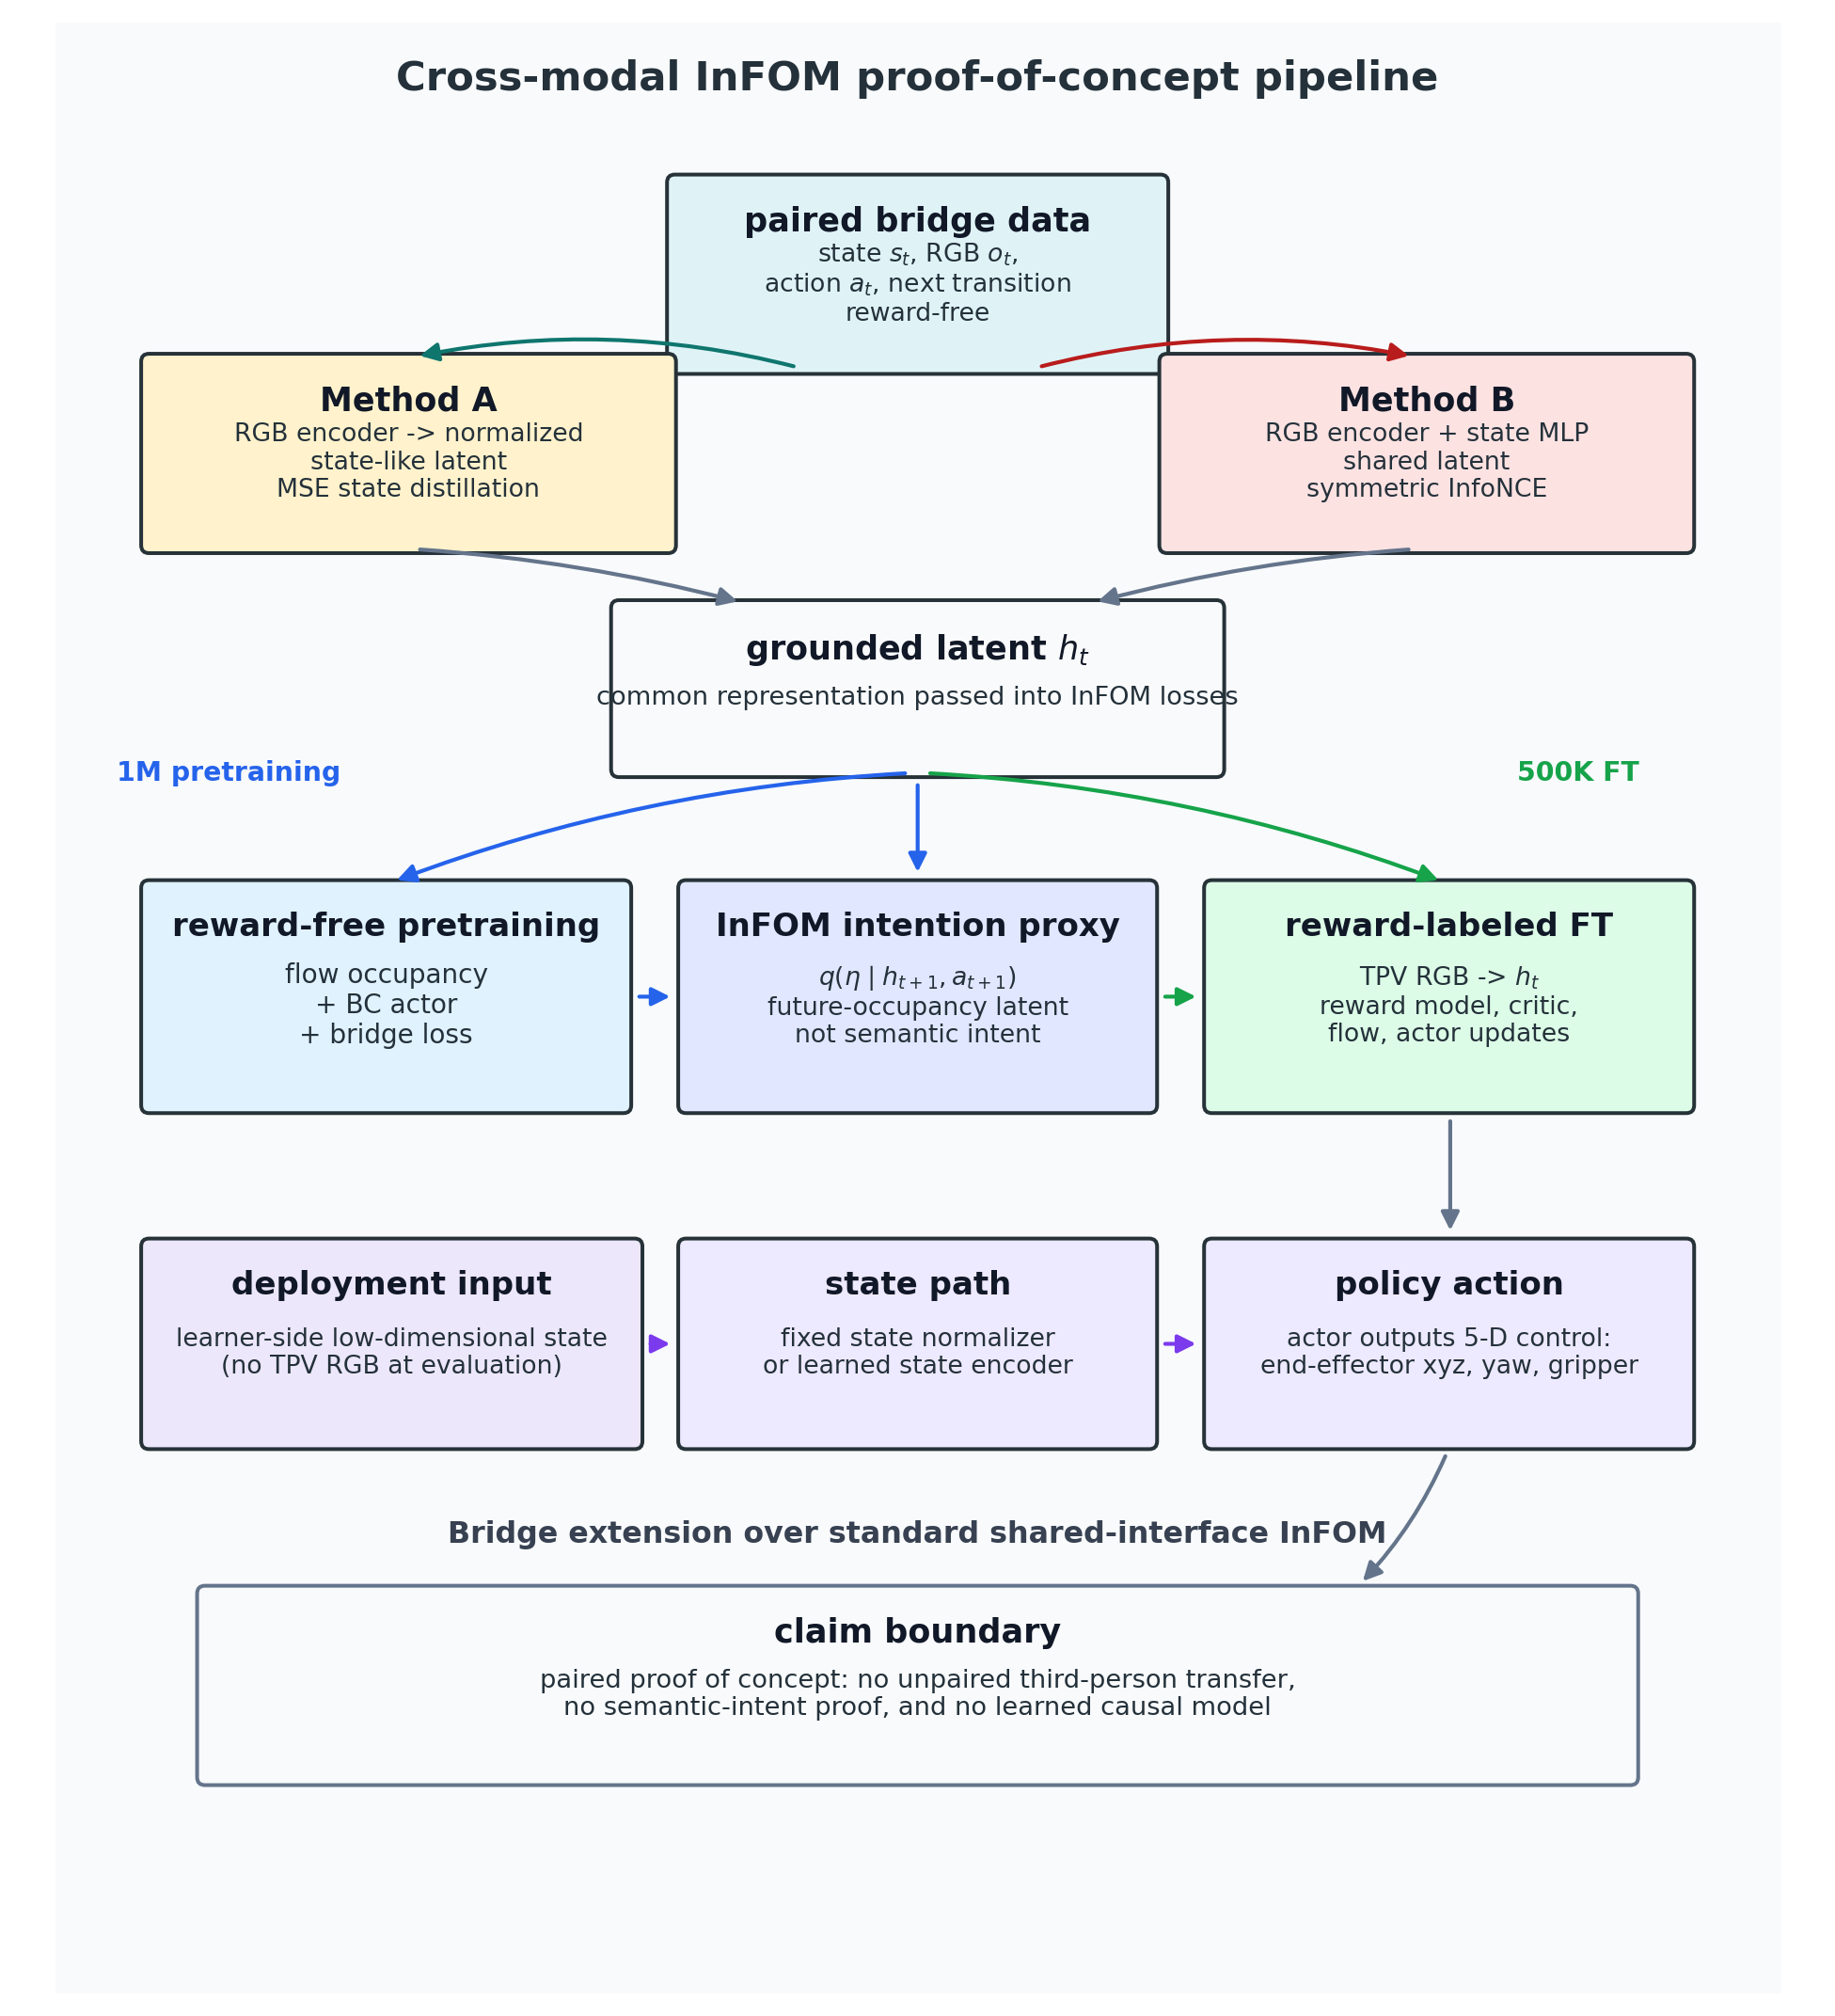
\includegraphics[width=\linewidth]{cross_modal_infom_architecture.png}
    \caption{Cross-modal InFOM pipeline. Reward-free paired state/RGB pretraining trains one of two bridges: Method A distills TPV RGB into a normalized state-like latent, while Method B aligns RGB and state encoders with symmetric InfoNCE. Reward-labeled fine-tuning updates control components in the grounded latent space, and deployment samples actions through the learner-side state path.}
    \label{fig:cross-modal-architecture}
\end{figure}

\section{Evaluations}
\label{sec:evaluations}

The evaluation asks whether reward-free pretraining learns a usable bridge, whether fine-tuning can turn that bridge into useful behavior at any checkpoint, and whether the behavior survives the final reporting window. Following the InFOM OGBench protocol, final-window success averages evaluation success at 400K, 450K, and 500K fine-tuning steps \citep{Zheng2025InFOM}. Since all report runs resume from 1M reward-free pretraining steps, these correspond to total training steps 1.4M, 1.45M, and 1.5M. Best-checkpoint success is the maximum observed checkpoint success, and the best-to-final-window gap measures instability. Uncertainties are standard errors across runs.

Bridge data were generated in OGBench cube-single using the local play-oracle data script. Each transition records learner-side state, action, terminal/simulator fields, and a synchronized TPV RGB render from the \texttt{front\_pixels} camera. Separate reward-free pretraining and fine-tuning bridge splits were generated through the same path and loaded with OGBench-style single-task reward relabeling. Tasks 1--5 are five fixed reward relabelings in the same cube-single domain: they share robot, action space, and bridge format, but evaluate different cube manipulation goals.

Reported runs use 1M reward-free pretraining gradient steps on paired state/RGB transitions and 500K fine-tuning steps on reward-labeled TPV transitions. In fine-tuning, both methods update control components in the grounded latent space; evaluation samples actions through the learner-side state path. Evaluation uses 50 episodes every 50K fine-tuning steps, with checkpoints saved every 50K steps. The audit contains 47 complete final-window run rows across Method A and Method B variants generated through the same local scripts and aggregation pipeline. Runs were launched on the Unity Slurm cluster as single-GPU jobs; representative fine-tuning jobs took about 45--90 minutes on L40S or A100-class GPUs.

The InFOM numbers in Table~\ref{tab:method-a-tasks} are paper-reported state-based OGBench cube-single final-window means, not reproduced local baselines. They provide scale for the original shared-interface target, while Method A/B comparisons are more direct because they use the same bridge data and aggregation pipeline.

\subsection{Method A Versus Contextual Paper Targets}

\begin{table}[H]
    \centering
    \small
    \caption{Method A task-level results. Means include standard error. The InFOM column is paper-reported context, not a reproduced local baseline.}
    \label{tab:method-a-tasks}
    \begin{tabular}{rrrrr}
        \toprule
        Task & Runs & Final-window mean & Best mean & InFOM final-window mean \\
        \midrule
        1 & 5 & $0.191 \pm 0.133$ & $0.656 \pm 0.062$ & 0.925 \\
        2 & 2 & $0.013 \pm 0.013$ & $0.170 \pm 0.070$ & 0.784 \\
        3 & 2 & $0.123 \pm 0.123$ & $0.360 \pm 0.000$ & 0.564 \\
        4 & 6 & $0.199 \pm 0.090$ & $0.477 \pm 0.077$ & 0.915 \\
        5 & 2 & $0.017 \pm 0.017$ & $0.480 \pm 0.080$ & 0.700 \\
        \bottomrule
    \end{tabular}
\end{table}

Table~\ref{tab:method-a-tasks} shows the main positive signal: Method A finds useful best checkpoints on tasks 1 and 4. Task 5 also reaches a high best mean, but its near-zero final-window mean makes it evidence of instability rather than robust task success. Overall, the results support a paired-bridge control signal, not performance superiority over InFOM.

\begin{figure}[htbp]
    \centering
    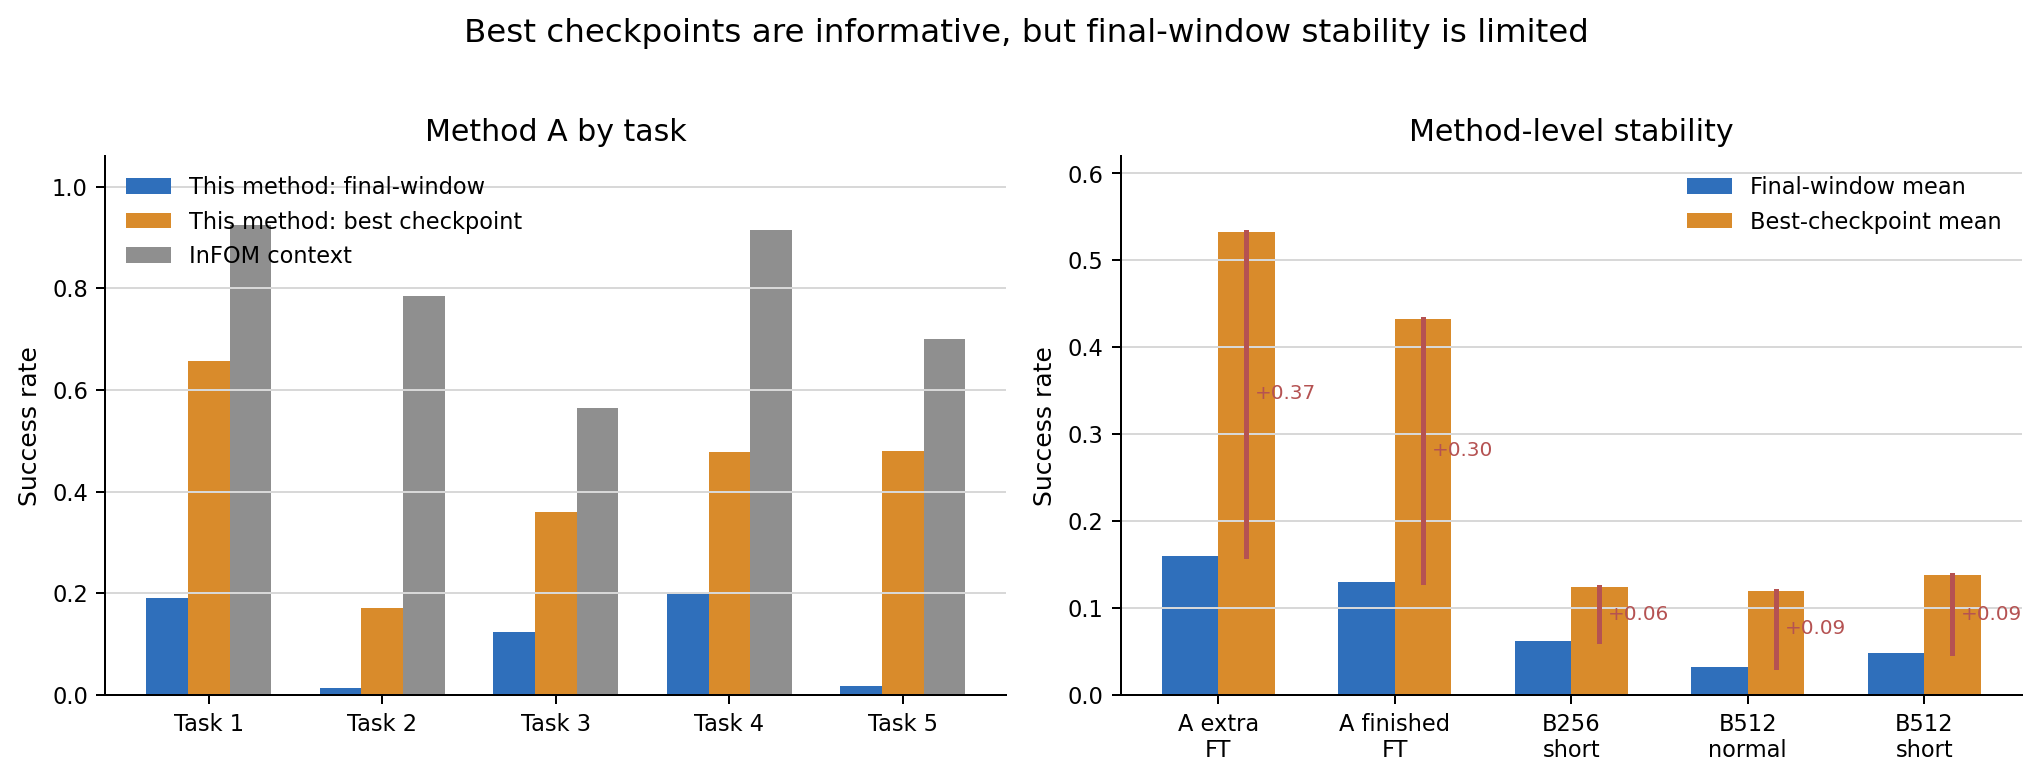
\includegraphics[width=\linewidth]{central_success_comparison.png}
    \caption{Central success comparison. Method A has stronger best-checkpoint signals than Method B, but also larger best-to-final-window gaps.}
    \label{fig:central-results}
\end{figure}

\subsection{Stability and Method Comparison}

Method B is reported with 256- and 512-dimensional contrastive state/RGB latents. All rows use the same reward-free pretraining, reward-labeled fine-tuning, and learner-side state evaluation structure; the ``short fine-tuning pack'' rows are additional Method B runs from the same aggregation pipeline.

\begin{table}[H]
    \centering
    \small
    \caption{Method-level comparison. Means include standard error; gap is best mean minus final-window mean.}
    \label{tab:stability}
    \begin{tabularx}{\linewidth}{Xrlll}
        \toprule
        Method/source & Runs & Final-window mean & Best mean & Gap \\
        \midrule
        A, extra fine-tuning seeds & 8 & $0.160 \pm 0.087$ & $0.533 \pm 0.076$ & 0.373 \\
        A, finished fine-tuning grid & 9 & $0.130 \pm 0.064$ & $0.433 \pm 0.064$ & 0.303 \\
        B 256, short fine-tuning pack & 10 & $0.062 \pm 0.013$ & $0.124 \pm 0.019$ & 0.062 \\
        B 512, normal fine-tuning & 10 & $0.032 \pm 0.009$ & $0.120 \pm 0.014$ & 0.088 \\
        B 512, short fine-tuning pack & 10 & $0.048 \pm 0.013$ & $0.138 \pm 0.024$ & 0.090 \\
        \bottomrule
    \end{tabularx}
\end{table}

Table~\ref{tab:stability} shows the central tradeoff. Method A produces stronger best-checkpoint behavior than Method B, but with a larger best-to-final-window gap. Method B is weaker overall; its smaller gap partly reflects that it never reaches comparable best success.

\subsection{Pretraining Diagnostics}

Pretraining diagnostics matter because this is where observational grounding is supposed to happen. For Method A, RGB/state alignment loss decreased from 0.620 to 0.396 between the first-10 and last-10 validation means; RGB/state actor action cosine improved from 0.683 to 0.917; flow matching loss decreased from 0.0240 to 0.0084; negative ELBO decreased from 0.201 to 0.0097; and KL loss decreased from 3.545 to 0.024.

Method B gives the clearest negative lesson. Both the 256- and 512-dimensional variants reached 1.0 RGB-to-state and state-to-RGB retrieval accuracy at 1M pretraining steps, with action cosine agreement around 0.96. The failure was therefore not cross-modal alignment under the pretraining objective; strong retrieval alignment did not reliably become a control-useful representation after fine-tuning.

Fine-tuning diagnostics were used as instability checks rather than as headline evidence. Return, reward, critic, actor, flow, gradient, and runtime traces varied across runs. These diagnostics are consistent with unstable offline fine-tuning, but they do not isolate a causal mechanism for the best-to-final-window gap.

\section{Discussion and Limitations}

The original hypotheses are only partly tested. H1 remains open because the system still relies on paired bridge data with state, RGB, and actions. H2 has weak-to-moderate support: Method A grounds TPV RGB into a learner-side state-like latent and supports some downstream control, but no probe shows that the latent captures strategy rather than state reconstruction or viewpoint correspondence. H3 is inconclusive: Method A beats Method B in available within-project comparisons, but final-window success is unstable and clean state-only or non-intent baselines are incomplete.

The main result is modest but useful: reward-free pretraining can be used as the stage where paired cross-modal grounding produces control-useful signals inside an InFOM-style latent-intention pipeline. The evidence is strongest for Method A. Method B shows the corresponding negative result: near-perfect retrieval alignment is not enough when the downstream policy still fails to control well. For observational learning, the pretraining objective must preserve effect- or intent-relevant structure for control, not merely match paired observations.

The main empirical limitation is fine-tuning instability. Method A often finds promising checkpoints, but final-window success is much weaker, so future work should stabilize downstream offline RL before making broad transfer claims \citep{Levine2020OfflineRL}. The remaining limitations fall into three groups:
\begin{itemize}[leftmargin=1.5em]
    \item \textbf{Evidence limits:} seed coverage is modest, exact InFOM reproduction is not established, and contextual InFOM numbers are paper targets rather than local baselines.
    \item \textbf{Scope limits:} the method requires exact paired state/RGB correspondence, does not test unpaired third-person observations, and has only been evaluated on OGBench cube-single.
    \item \textbf{Conceptual limits:} no formal causality or action-effect model is learned, semantic intent is not directly proven, and the \texttt{impala\_small} visual encoder may be weaker than pretrained robotics representations such as R3M \citep{Nair2023R3M}.
\end{itemize}

\begin{table}[H]
    \centering
    \small
    \caption{Original goals versus completed evidence.}
    \label{tab:completed}
    \begin{tabularx}{\linewidth}{p{0.25\linewidth}p{0.16\linewidth}X}
        \toprule
        Original goal & Status & Evidence and boundary \\
        \midrule
        Learn from observation, not only reward learning & Partial & Pretraining learned RGB/state grounding and InFOM flow/intent structure, but still required paired bridge data and actions. \\
        Infer reusable intent & Proxy & InFOM latent intention is an implementable proxy, not semantic intent or causal effect inference. \\
        Bridge third-person observation to learner control & Partial & Method A produced useful best-checkpoint signals, but not unpaired or cross-embodiment transfer. \\
        Improve over baselines & Inconclusive & Method A outperformed Method B using the same local scripts, but reproduced InFOM baselines are missing. \\
        Learn causality/effects & Not completed & Causality is only a motivating idea and future direction. \\
        \bottomrule
    \end{tabularx}
\end{table}

\section{Conclusion and Future Work}

The final result is a proof of concept for observational learning with intent-like representations. A paired RGB/state bridge learned during reward-free pretraining can feed an InFOM-style offline RL pipeline and produce useful but unstable control signals. This extends InFOM toward cross-modal observation-to-control learning, but remains short of robust intent transfer, cross-embodiment observational learning, or causal goal inference.

The next steps I would prioritize are:
\begin{itemize}[leftmargin=1.5em]
    \item stabilize fine-tuning with stronger regularization, reward/critic checks, checkpoint selection, and cleaner local InFOM reproduction;
    \item ablate state distillation, contrastive alignment, behavior cloning, and flow-occupancy losses to test which pretraining signals support downstream control;
    \item remove the exact paired bridge assumption and test true third-person observation transfer;
    \item probe whether learned latents encode goals/effects rather than viewpoint or state reconstruction, then add explicit effect or causal models for reasoning about which actions caused observed state changes;
    \item evaluate on broader OGBench tasks and eventually real robot settings, including failed demonstrations where the attempted goal is informative even if execution fails.
\end{itemize}

\begingroup
\raggedright
\setlength{\emergencystretch}{3em}
\bibliographystyle{plainnat}
\bibliography{references}
\endgroup

\end{document}
